% Generated by tex/build_swebok_structure.py from tex/chapters/ch01/06_要求仕様化.tex
\subsubsection{モデルに基づく要求仕様化}

\term{モデル}とは、複雑な対象を理解しやすくするために、必要な部分だけを抽象化して表したものです。要求仕様化では、文章だけでなく、図や形式的な記法を使って要求を表すことがある。UMLやSysMLの一部は、そのために使われる。

モデルは大きく二種類に分けられる。\term{構造モデル}は、概念、データ、関係、業務規則を表す。\term{振る舞いモデル}は、処理の流れ、利用者とのやり取り、状態遷移、イベントへの反応を表す。

\par\smallskip\noindent\refstepcounter{table}\label{tab:ch01-10}\textbf{表 \thetable: 第01章 ソフトウェア要求 表10}\par\smallskip
\begin{tabularx}{0.97\linewidth}{@{}p{.24\linewidth}X@{}}
\toprule
モデルの種類 & 例 \\
\midrule
構造モデル & クラス図、概念データモデル、実体関連図。 \\
振る舞いモデル & ユースケース図、シーケンス図、状態遷移図、活動図、データフロー図。 \\
\bottomrule
\end{tabularx}

モデルには、手描きのラフな図から、数学的意味を厳密に持つ形式モデルまで幅がある。形式性が高いほど曖昧さは減るが、作成と理解の負担は増える。

\begin{figure}[htbp]
\centering
\IfFileExists{assets/generated_figures/ch01/fig-ch01-08.png}{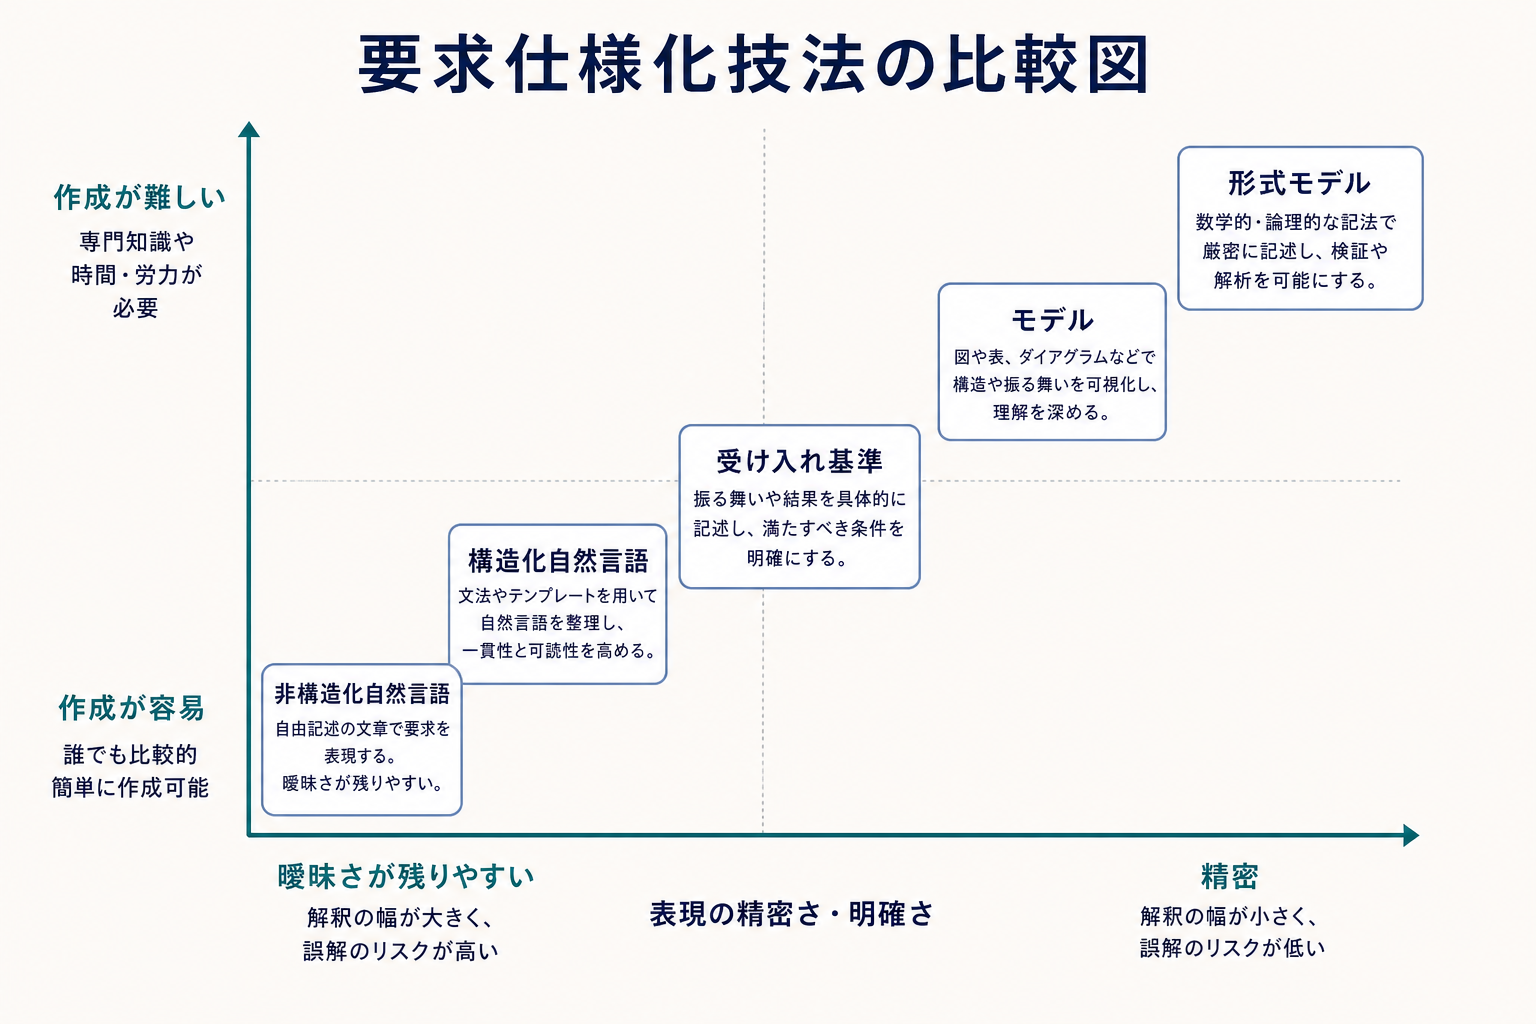
\includegraphics[width=0.96\linewidth]{assets/generated_figures/ch01/fig-ch01-08.png}}{\fbox{\parbox[c][48mm][c]{0.9\linewidth}{\centering 画像生成待ち\\要求仕様化技法の比較図}}}
\caption{要求仕様化技法の比較図}
\label{fig:ch01-08}
\end{figure}
